%!TEX root = base.tex

\chapter{Background}

This report touches a wide range of topics, technologies and systems, and this
chapter briefly introduces them and provides a summary of their, for this
report, key points.

\section{IEEE 802.11}

The now ubiquitous family of wireless network protocols and ammendments, such
as IEEE 802.11g and IEEE 802.11x, commonly known as Wi-Fi. More specifically
IEEE 802.11 defines the PHY and MAC layers of the network stack. Each
ammendment introduces additions, redactions and changes to these layers. It's
best to read the following overview with this in mind. For a more complete
definition of the \emph{distributed coordination function} (DCF) the reader is
referred to \cite{654749}, \cite{5307322} and \cite{6687187}. 

IEEE 802.11 implements a \emph{Carrier-Sense Multiple Access} (CSMA) medium
access control (MAC) scheme with a binary exponential backoff algorithm for
\emph{collision avoidance} (CA). The algorithm is run locally on each network
node and is called the \emph{Distributed Coordination Function} (DCF). 

When nodes in a IEEE 802.11 network wants to transmit data they must first
listen on the channel and wait until no activity has been detected for a
duration, the \emph{DCF Interframe Space} (DIFS). Since this effectively
synchronizes the nodes waiting to transmit, a random delay is introduced to
desynchronise nodes. This delay is called back-off time
($T_{\mathit{backoff}}$) and belongs to the \emph{collision avoidance}
algorithm which requires time to be quantized into discrete \emph{time-slots},
each $9$ to $50$ $\mu s$ long, depending on the standard. 

While in back-off, nodes listen on the medium for a full \emph{slot} and, if
no activity has been sensed, decrements the back-off counter. If nodes detect
activity on the medium during a slot, the counter is not decremented (counter
freezing). Upon reaching zero the node may attempt to (re)transmit. If no
\texttt{ACK} has been received after a certain duration (\texttt{ACK-Timeout})
the node waits another DIFS, enters further back-off (see \ref{fig:cwsizes})
and restarts its journey back to zero again. The node has a fixed number of
attempts to retransmit the frame, \texttt{ShortRetryLimit} \cite{654749}, and
drops the frame once exceeded.

\begin{figure}
\center
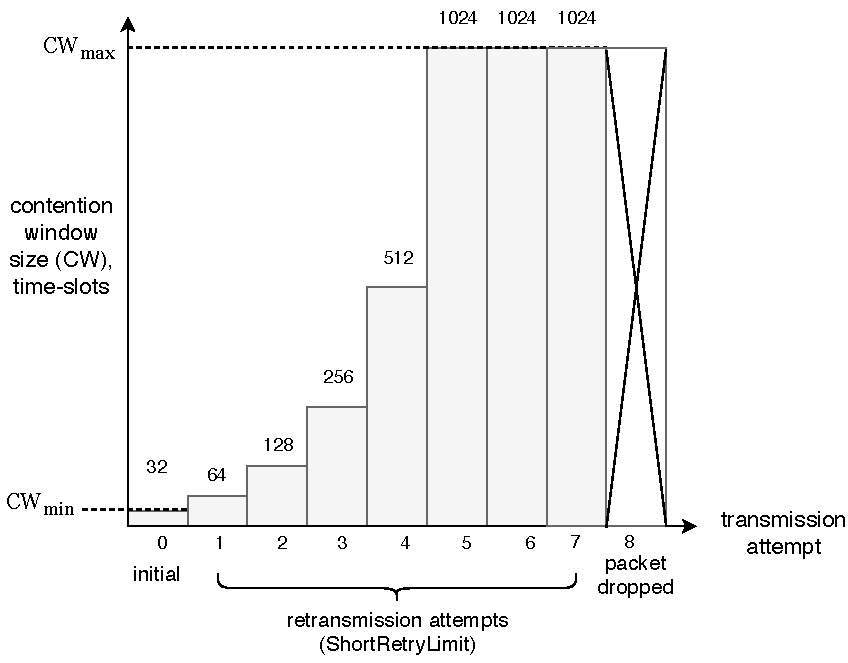
\includegraphics[width=0.8\textwidth]{images/contention-window-sizes.pdf}
\caption{Contention window size increases exponentially on each retransmission attempt, from $\mathit{CW}_{min}$ up to $\mathit{CW}_{max}$}
\label{fig:cwsizes}
\end{figure}

Time spent in back-off for each (re)transmission attempt $j$ is described in
equation \ref{eq:tbackoff}, where \emph{SlotTime} is defined in \cite{654749}
and $\mathcal{U}(0,W_j-1)$ is a uniformly sampled value between $0$ and the
\emph{contention window size} $W_{j}-1$, i.e. the maximum number of
time-slots (exclusive, since 0 is a valid back-off counter). 

The \emph{contention window size} at transmission attempt $j$, $W_{j}$, is
defined in equation \ref{eq:cwj}, where $L$ is the number of retransmssion
attempts before a packet is dropped (\texttt{ShortRetryLimit}),
$\mathit{CW}_{min}$ and $\mathit{CW}_{max}$ are minimum and maximum number of
time-slots of the \emph{contention window}, respectively, and $m$ is $\log_2
\frac{\mathit{CW}_{max}}{\mathit{CW}_{min}}$. The defined values of $j$ are
the initial attempt ($j=0$) and an extra $L$ attempts before termination,
which resolves to $0 \leq j \leq L$.

\begin{equation} \label{eq:tbackoff}
T^j_{\mathit{backoff}} = \mathit{SlotTime} \times \mathcal{U}(0,W_j-1)
\end{equation}

\begin{equation} \label{eq:cwj}
W_j = \left\{
	\begin{array}{ll}
		2^j \mathit{CW}_{min}  & \mbox{if } 0 \leq j < m, \\
		\mathit{CW}_{max}      & \mbox{if } m \leq j \leq L
	\end{array}
\right.
\end{equation}

The description above details one of three multiple access schemes in IEEE
802.11—``basic mode''. During CSMA/CA each node listens for activity locally
and can therefore fail to detect nodes whose signal is too weak to be
received, causing what's known as the \emph{hidden node} problem. In
IEEE 802.11, only the access point (AP) is guaranteed to have knowledge of all
connected stations (STAs). The second multiple access scheme requires that
STAs first acquire the right to transmit, using a \emph{request-to-send} (RTS)
message. If the STA is given permission, the AP will respond with a
\emph{clear-to-send} (CTS) message. This access scheme is called RTS/CTS and
increases performance in scenarios with multiple ``hidden nodes''. [TODO REF?]

\section{TG799-vac}

The OpenWrt-based router examined in this thesis, see Figure \ref{fig:tg799}, is
commonly known as TG799, manufactured by Technicolor with Broadcom and Quantenna
modems. It is, as of time of writing, the default router provided by many
Swedish ISPs, and therefore widely deployed.

A custom firmware was used to gain root access.

\begin{figure}
\center
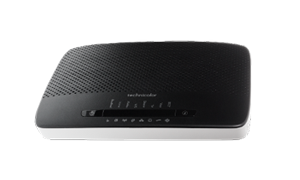
\includegraphics[width=0.5\textwidth]{images/tg799.png}
\caption{The TG799 router from Technicolor}
\label{fig:tg799}
\end{figure}

\section{ubus - the OpenWrt micro bus architecture}

A client program which acts as an interface to the bus daemon, \texttt{ubusd}.
Input and output format is JSON.

\section{Deutche telekom supra}

Björns oklara vapen.

\section{Rhode \& Schwarz FWLZ-XYZ}

(not broken) network analyser;

\section{Wi-Spy Channalyzer}

the wi-spy, top secret agent auf d00m.

\section{Wireshark, tshark}

Wireshark is a well-known program for capturing and inspecting network data
based around \texttt{libpcap}.

\section{jana}

A program, developed by the author of this thesis, for running network tests.
Supports expontential, uniform and gamma distributed packet send rate and
payload size. It is designed to be used together with packet capture software
(e.g. Wireshark) which enables a user to estimate the time from a `sendmsg`
syscall to the packet actually leaving the NIC. These features were developed
to facilitate experimental, yet controlled, evaluation of the theoretical IEEE
802.11 performance models.

\section{Linux Networking}

A high level view of a packet's way from the userspace program, through the
kernel and finally to the network interface responsible for physically
transmitting it can be found in \ref{fig:linux_egress}.

\begin{figure}
\center
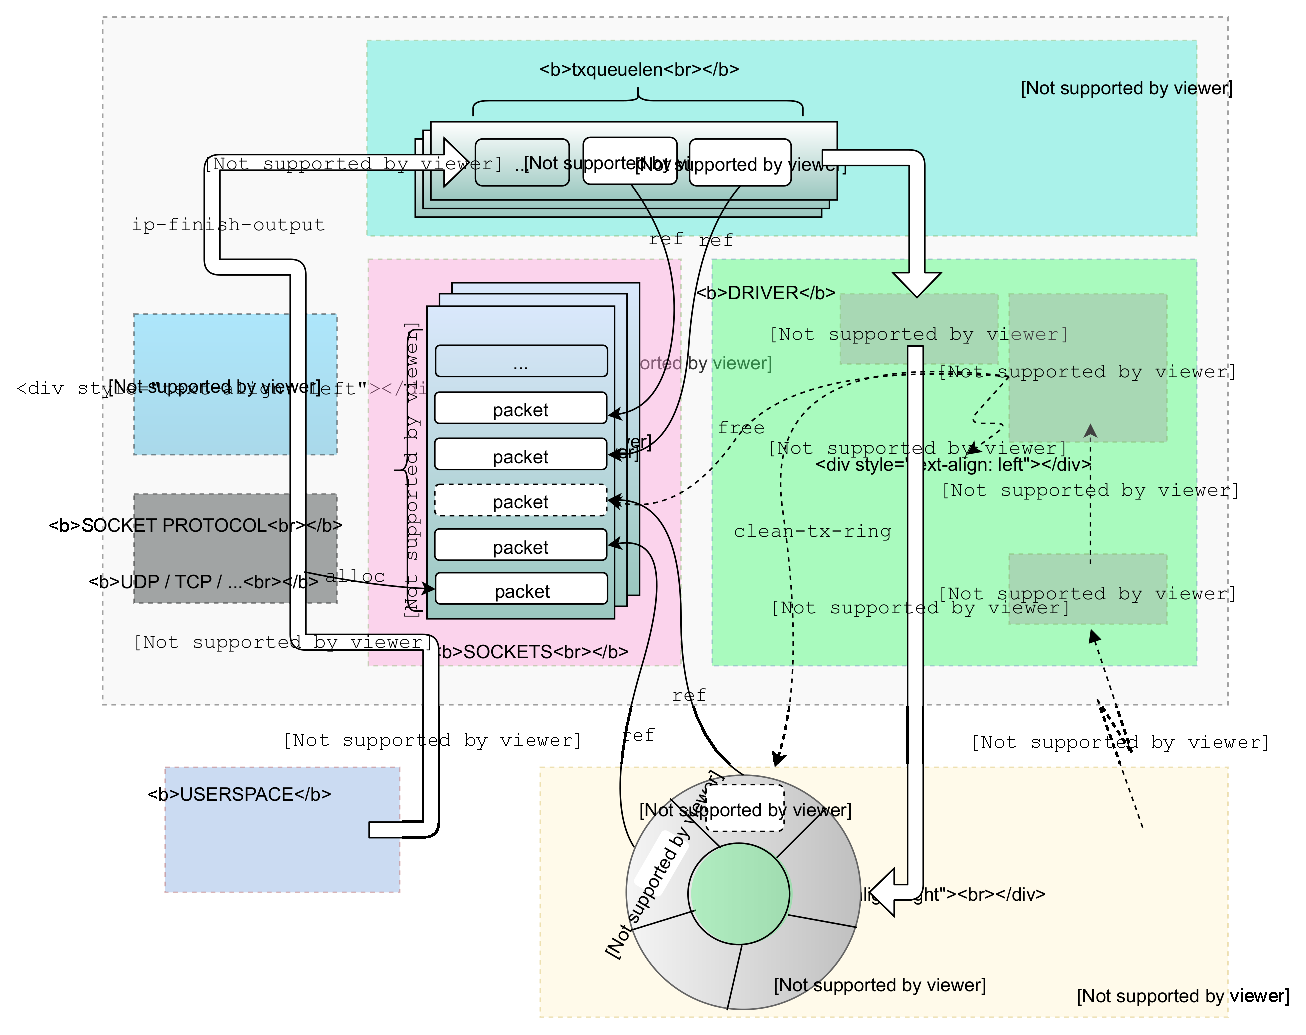
\includegraphics[width=0.9\textwidth]{images/linux-egress-overview.eps}
\caption{TG799 router and measurement antenna side by side, 1 meter from laptop}
\label{fig:linux_egress}
\end{figure}
